\documentclass{article}
\usepackage{graphicx}
\usepackage[brazilian]{babel}
\usepackage[utf8]{inputenc}
\usepackage[T1]{fontenc}
\usepackage{amsmath}
\usepackage{amssymb}
\setlength{\parindent}{0in}

\begin{document}
	
	\title{Lista 2 - Otimização Não Linear}
	\author{Daniel Yoshio Hotta – 9922700}
	
	\maketitle	
	
	\textbf {E2} 
	\\ \\
	\textit {Considerações iniciais:} \\
	
	\begin{center}
		$M$ = média das observações ${x_1, x_2, ..., x_n}$\\
		$m$ = mediana das observações ${x_1, x_2, ..., x_n}$\\
		$dp$ = desvio padrão das observações ${x_1, x_2, ..., x_n}$\\
	\end{center}
	
	\textbf {E2.a} 
	\\ \\
	\textit {Resposta:} \\
	
	Teremos todos os valores multiplicados por 2, logo:\\
	
	Conjunto de dados:\\
	
	${2x_1, ..., 2x_n}$\\
	
	\textbf {Média:}\\
	
	$M_a = \frac{2x_1 + 2x_2 + ... + 2x_n}{n} = 2 . \frac{x_1 + x_2 + ... + x_n}{n} = 2M$\\
	
	\textbf {Mediana:}\\
	
	Caso ímpar: $m_a = 2m$ (pois é só pegar o termo do meio após ordenação)\\
	
	Caso par: $m_a = \frac{2x_i + 2x_{i+1}}{2} = 2 \frac{x_i + x_{i+1}}{2} = 2m$ (com $x_i, x_{i+1}$ sendo os valores no meio após a ordenação.)\\
	
	\textbf {Desvio Padrão:}\\
	
	$dp_a = \sqrt{\frac {\sum (2x_i - M_a)^2}{n}} = \sqrt{\frac {\sum (x_i - M)^2.2^2}{n}} = 2. \sqrt{\frac {\sum (x_i - M)^2}{n}} = 2dp$\\
	
    
    
    
    
	
	\textbf {E2.b} 
	\\ \\
	\textit {Resposta:} \\
	
	Teremos todos os valores acrescidos de 10, logo:\\
	
	Conjunto de dados:\\
	
	${x_1 + 10, ..., x_n + 10}$\\
	
	\textbf {Média:}\\
	
	$M_b = \frac{x_1 + 10 + x_2 + 10 + ... + x_n + 10}{n} = \frac{x_1 + x_2 + ... + x_n + 10n}{n} = 10 + \frac{x_1 + x_2 + ... + x_n}{n} = 10 + M$\\
	
	\textbf {Mediana:}\\
	
	Caso ímpar: $m_b = m + 10$ (pois é só pegar o termo do meio após ordenação)\\
	
	Caso par: $m_b = \frac{x_i + 10 + x_{i+1} + 10}{2} = \frac{20 + x_i + x_{i+1}}{2} = m + 10$ (com $x_i, x_{i+1}$ sendo os valores no meio após a ordenação.)\\
	
	\textbf {Desvio Padrão:}\\
	
	$dp_b = \sqrt{\frac {\sum (x_i + 10 - M_b)^2}{n}} = \sqrt{\frac {\sum (x_i + 10 - (M + 10))^2}{n}} = \sqrt{\frac {\sum (x_i - M)^2}{n}} = dp$\\
	
	\textbf {E2.c} 
	\\ \\
	\textit {Resposta:} \\
	
	Teremos todos os valores subtraídos $\bar{x}$ (no nosso caso, M), logo:\\
	
	Conjunto de dados:\\
	
	${x_1 - M, ... , x_n - M}$\\
	
	\textbf {Média:}\\
	
	$M_c = \frac{x_1 - M + x_2 - M + ... + x_n - M}{n} = \frac{x_1 + x_2 + ... + x_n - Mn}{n} = -M + \frac{x_1 + x_2 + ... + x_n}{n} = \\  \\
	-M + M = - \bar{x} + \bar{x} = 0$\\
	
	\textbf {Desvio Padrão:}\\
	
	$dp_c = \sqrt{\frac {\sum (x_i - M - M_c)^2}{n}} = \sqrt{\frac {\sum (x_i - M - 0))^2}{n}} = \sqrt{\frac {\sum (x_i - \bar{x})^2}{n}} = dp$\\
	
	\textbf {E2.d} 
	\\ \\
	\textit {Resposta:} \\
	
	Teremos todos os valores subtraídos $\bar{x}$ (no nosso caso, M), logo:\\
	
	Conjunto de dados:\\
	
	$\frac{x_1 - M}{dp}, ... , \frac{x_n - M}{dp}$\\
	
	\textbf {Média:}\\
	
	$M_d = \frac{\frac{x_1 - M}{dp} + ... + \frac{x_n - M}{dp}}{n} = \frac{x_1 + x_2 + ... + x_n - Mn}{n.dp} = \frac{-M}{dp} + \frac{x_1 + x_2 + ... + x_n}{n.dp} = \\  \\
	\frac{-M}{dp} + \frac{M}{dp} = 0$\\
	
	\textbf {Desvio Padrão:}\\
	
	$dp_c = \sqrt{\frac {\sum (\frac{x_i - M}{dp} - M_c)^2}{n}} = \sqrt{\frac {\sum (\frac{x_i - M}{dp} - 0))^2}{n}} = \sqrt{\frac {\sum (x_i - \bar{x})^2}{n.dp^2}} =\\ \\
	= \frac{1}{dp} . \sqrt{\frac {\sum (x_i - \bar{x})^2}{n}} = 1$\\
	
	\textbf {E4.a} 
	\\ \\
	\textit {Resposta:} \\
	
	$IQR_A = Q1_A - Q3_A = 22,68 - 17,32 = 5,36$\\
	
	$Q1_A - 1,5 . IQR_A =  17,32 - 8,04 = 9,28$\\
	
	$Q3_A - 1,5 . IQR_A = 22,68 + 8,04 = 30,72$\\
	
	\begin{figure}[h]
		\caption{Exercício 4.a}
		\centering % para centralizarmos a figura
		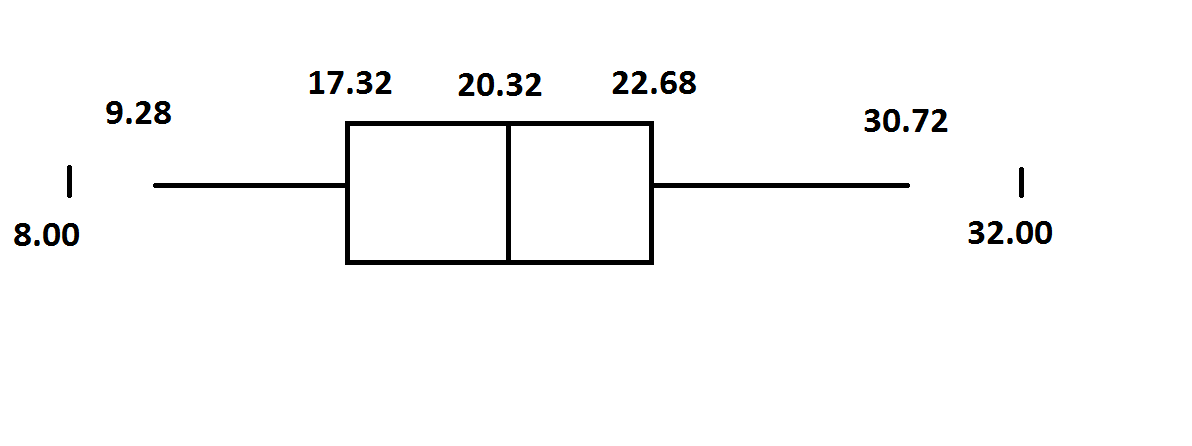
\includegraphics[width=16cm]{q4a-a.png} % leia abaixo
		\label{figura: Região A}
	\end{figure}

    
	
\end{document}
